\section{Front-End Mock Up}

In the previous milestones we already created a frond-end in order to provide an interactive visualization of our collected datasets. This front-end was built using python dash, a framework that builds on top of Flask and React. The respective webserver is deployed by use of Heroku and can be found at the following URL: \url{https://ami-group1-dashboard.herokuapp.com/}.

In order to present our final results, the same framework will be used. In particular, the website will be divided into multiple sections. Our goal is to use the front-end in order to show what datasets were used, how the model pipeline is structured and of course to show the final conclusion in regard to the research question. The basic layout is shown in Figure \ref{fig:front_end_title_page}.

\begin{figure}[h!]
\centering
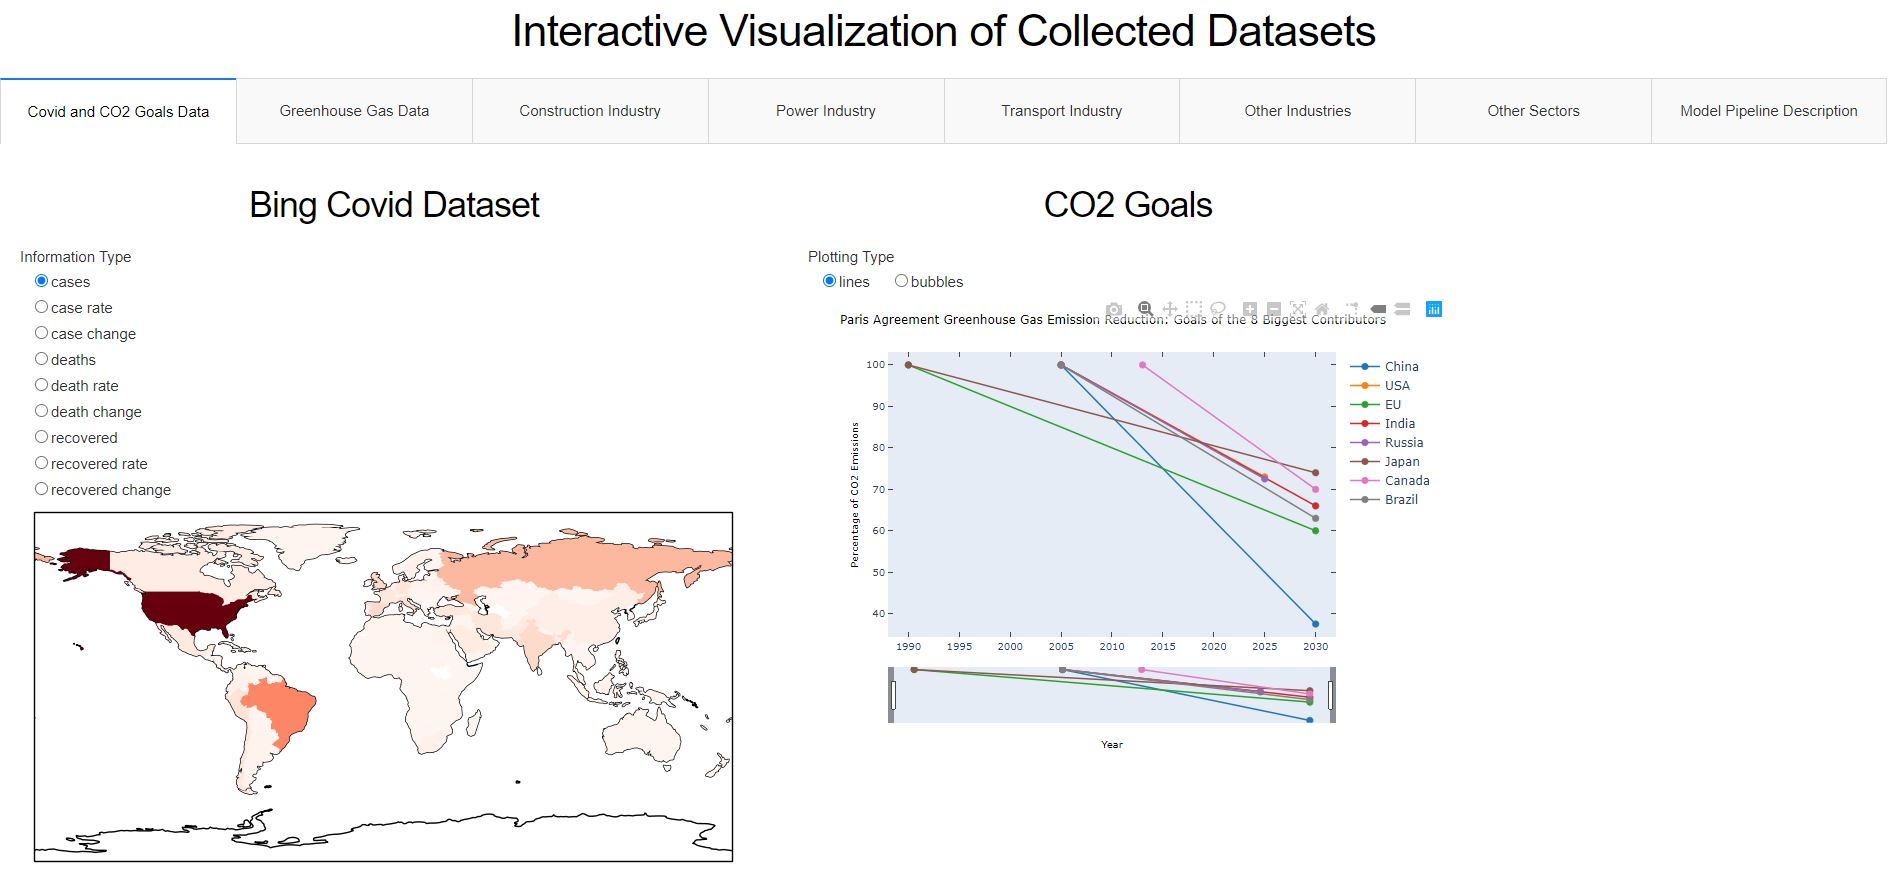
\includegraphics[width=0.9\textwidth]{front_end_title_page}
\caption{Frontend title page}
\label{fig:front_end_title_page}
\end{figure}

As shown above, the different sections are divided into COVID-19 data, greenhouse gas data and indicators for various industries. In order to get an intuition about what our model pipeline looks like, there will be a separate section which graphically describes the entire pipeline. A preliminary version for this can be seen in Figure \ref{fig:model_pipeline}.

\begin{figure}[h!]
\centering
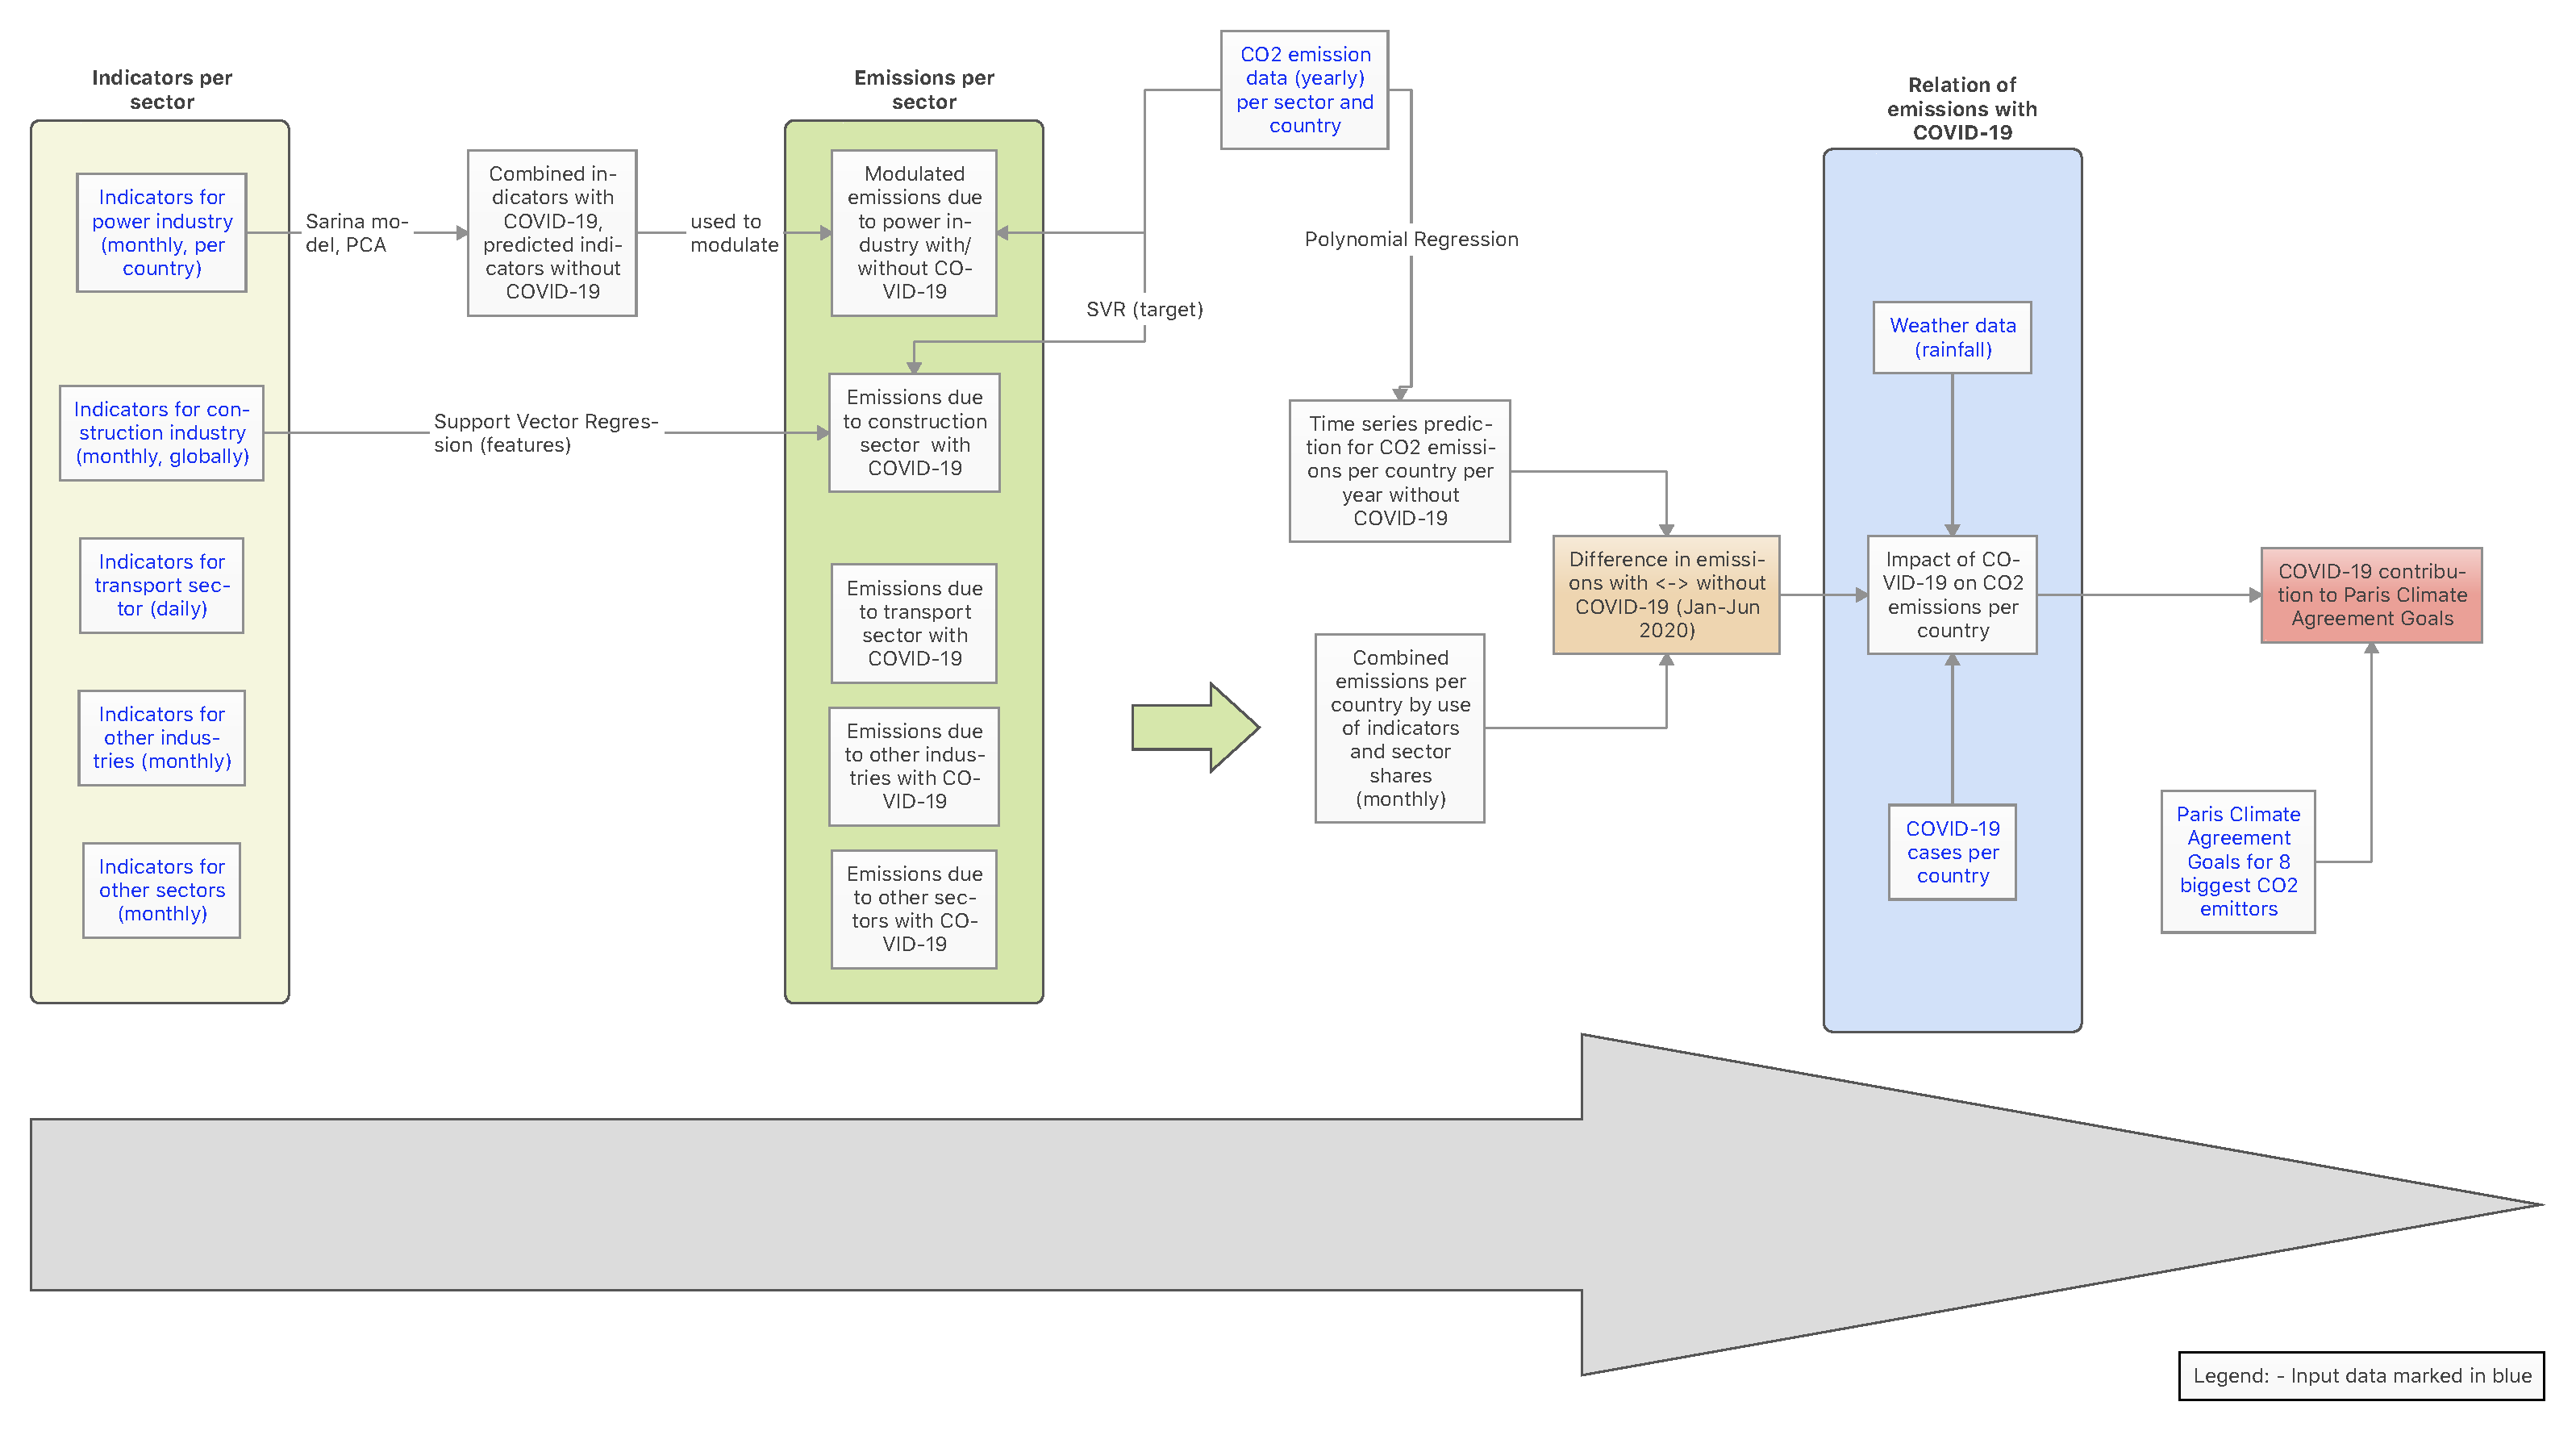
\includegraphics[width=0.9\textwidth]{mock-up_frontend_pipeline_description.pdf}
\caption{Model pipeline description}
\label{fig:model_pipeline}
\end{figure}

Finally, there will be a section showing our final results. In order to show the training-process, one possibility would be to let the model train while highlighting parts in the diagram shown above which are currently trained. This would be the most descriptive way we could provide our model pipeline to the reader. But since we use quite a variety of different models and some training steps require a lot of computational effort, this approach might not be feasible with regard to costs of the web instances we use, in this case provided by Heroku. This issue could be adressed by just partially training the model parts which are not that compuationally expensive.

On the other hand, there will not be significant advantages using a live-training approach compared to directly showing the results of pre-trained models. This is compuationally affordable for us and still can be done in an attractive way. Besides, the reader does not have to wait in order to get the results presented.

Those are the reasons why from the current point of view, we will not include live-training into our website. Still, we will try to keep it as interactive as possible. In particular, the reader should have the ability to select from different countries, inspect their CO2 emissions, the pandemic development and analyse the overall impact of COVID-19 on greenhouse gas emissions. Apart from that, we are planning to integrate some variability for the reader to hypothetically modify the impact of COVID-19. For example, one could then explore how the emissions would have behaved if COVID-19 had even more affected our daily lives in the first half of the year 2020. Another option could also be to explore how a second wave of COVID-19 in some specific countries, similar to the first one, could affect greenhouse gas emissions in the future.

Those interactive options, together with the final result of our research, will be shown on a last tab on the website (currently not available). Here we will present, for the biggest greenhouse gas emitting countries, the impact of COVID-19 on emissions which eventually will be compared to goals stated in the Paris Climate Agreement.

%Add a pointer to heroku page, add prediction plots and extracted information